\documentclass{beamer}
\usepackage{amssymb,amsmath}
\usepackage{graphicx}
\usepackage{url}
\usepackage{color}
\usepackage{pagenote}[continuous,page]
\usepackage{relsize}		% For \smaller
\usepackage{url}			% For \url
\usepackage{epstopdf}	% Included EPS files automatically converted to PDF to include with pdflatex

%For MindMaps
% \usepackage{tikz}%
% \usetikzlibrary{mindmap,trees,arrows}%

%%% Color Definitions %%%%%%%%%%%%%%%%%%%%%%%%%%%%%%%%%%%%%%%%%%%%%%%%%%%%%%%%%
%\definecolor{bordercol}{RGB}{40,40,40}
%\definecolor{headercol1}{RGB}{186,215,230}
%\definecolor{headercol2}{RGB}{80,80,80}
%\definecolor{headerfontcol}{RGB}{0,0,0}
%\definecolor{boxcolor}{RGB}{186,215,230}

%%% Save space in lists. Use this after the opening of the list %%%%%%%%%%%%%%%%
%\newcommand{\compresslist}{
%	\setlength{\itemsep}{1pt}
%	\setlength{\parskip}{0pt}
%	\setlength{\parsep}{0pt}
%}

%\setbeameroption{show notes on top}

% You should run 'pdflatex' TWICE, because of TOC issues.

% Rename this file.  A common temptation for first-time slide makers
% is to name it something like ``my_talk.tex'' or
% ``john_doe_talk.tex'' or even ``discrete_math_seminar_talk.tex''.
% You really won't like any of these titles the second time you give a
% talk.  Try naming your tex file something more descriptive, like
% ``riemann_hypothesis_short_proof_talk.tex''.  Even better (in case
% you recycle 99% of a talk, but still want to change a little, and
% retain copies of each), how about
% ``riemann_hypothesis_short_proof_MIT-Colloquium.2000-01-01.tex''?

\mode<presentation>
{
  \usetheme{CambridgeUS}
  \usecolortheme{dolphin}
  \useoutertheme{default}
  \useinnertheme{default}
  \setbeamercovered{invisible} % or whatever (possibly just delete it)
}
\beamertemplatenavigationsymbolsempty

\usepackage[english]{babel}
%\usepackage[latin1]{inputenc}
\usepackage{subfigure}

\usepackage{times}
\usepackage[T1]{fontenc}
\usepackage{CJKutf8}

%% makes the ppagenote command for figure references at the end.
\makepagenote
\renewcommand{\notenumintext}[1]{}
\newcommand{\ppagenote}[1]{\pagenote[Page \insertframenumber]{#1}}

\title[Experiment Design (01CH740)]{Experiment Design for Computer Sciences (01CH740)}
\author[Claus Aranha]{Claus Aranha\\{\footnotesize caranha@cs.tsukuba.ac.jp}}
\institute[U. Tsukuba]{University of Tsukuba, Department of Computer Sciences}


\subtitle[Experimentalism]{Topic 01 - What is an experiment?}

\begin{document}
\begin{CJK}{UTF8}{ipxm}

\begin{frame}
  \maketitle

  \vfill

  \hfill Version 2020.1
\end{frame}

%%%%%%%%%%%%%%%%%%%%%%%%%%%%%%%%%%%%%%%%%%%%%%%%%%%
\begin{frame}{Outline}
  \begin{itemize}
    \item What is Science?
    \item What is an Experiment?
    \item The characteristics of a good Experiment;
    \item Good experimental practices;
    \item Report 1 outline
  \end{itemize}
\end{frame}

\section{What is Science?}

\begin{frame}{What is Science?}
  As master degree students, what is science for you?
  \bigskip

  \begin{block}<2>{Answers from past years}
    \begin{itemize}
      \item A method to learn about the world;
      \item A method to reach the truth;
      \item Science is useful when it contributes to society;
      \item How we develop new technologies;
    \end{itemize}
  \end{block}
\end{frame}

\begin{frame}{Marie Curie}
  \begin{columns}
    \column{.3\textwidth}
  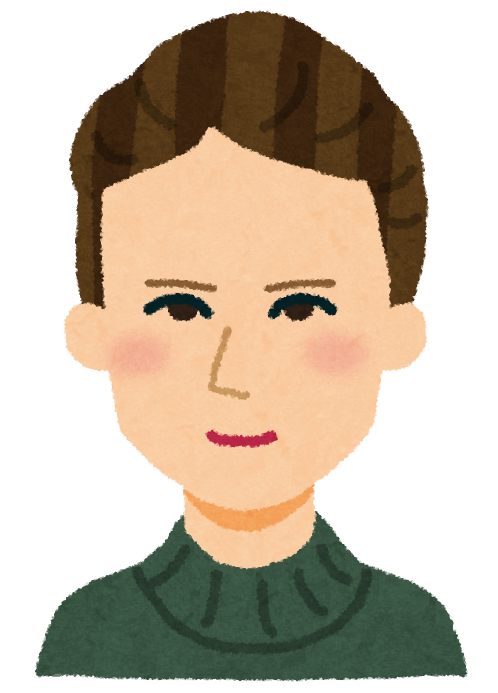
\includegraphics[width=1\textwidth]{../img/irasutoya_curie}
  \ppagenote{Marie Curie sketch from \url{https://www.irasutoya.com}}\\
    \begin{center}
      Marie Curie\\ 1867 -- 1934
    \end{center}
    \column{.7\textwidth}
    One way to learn about science, is to learn a little bit more about proeminent scientists.
    \bigskip

    {\bf Marie Curie}
    \begin{itemize}
      \item Physicist and Chemist
      \medskip

      \item Pioneer of radioactivity
      \medskip

      \item First woman to win the Nobel Prize
      \begin{itemize}
        \item First person to win the Nobel twice
      \end{itemize}
    \end{itemize}
  \end{columns}
\end{frame}

\begin{frame}{Marie Curie}{Humble Beginnings}
  \begin{columns}
    \column{0.3\textwidth}
    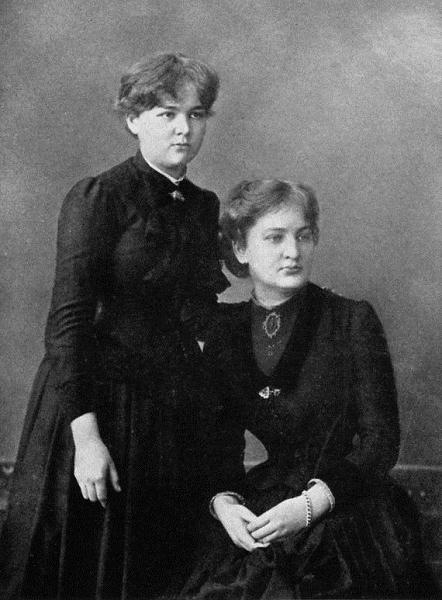
\includegraphics[width=1\textwidth]{../img/marie_curie_sister}\ppagenote{Curie sisters image from Wikipedia (public domain)}
    \column{0.7\textwidth}
  \begin{itemize}
    \item Born in Poland
    \medskip

    \item Could not enroll in a regular university because she was a woman, so she got educated at the clandestine "Flying University"
    \medskip

    \item Sustained herself working as a tutor and as a teacher for families;
  \end{itemize}
\end{columns}
\end{frame}

\begin{frame}{Marie Curie}{Moving to Paris}
  \hfill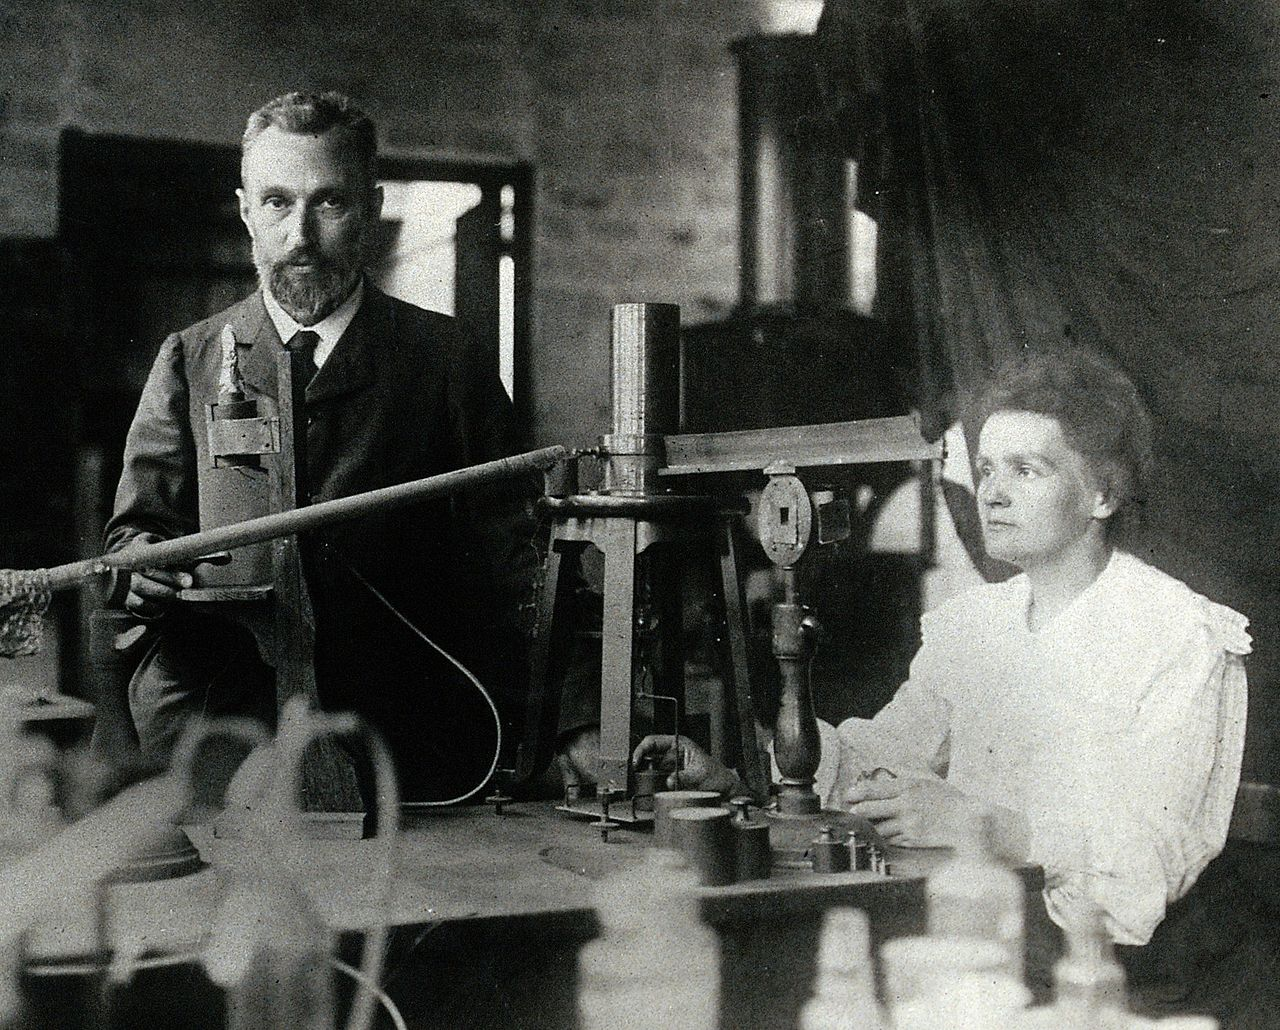
\includegraphics[width=.3\textwidth]{../img/marie_pierre_curie}\ppagenote{Marie and Pierre Curie image from Wikipedia (Public Domain)}
  \begin{itemize}
    \item Earned her Physics degree at the University of Paris

    \item Worked at a small shed and had difficulty acquiring funding;

    \item Found out that the emission of radiation from uranium
    depended only on the size of the sample;

    \item Did not patent her techniques, so science could proceed unimpeded;
  \end{itemize}
\end{frame}

\begin{frame}{Marie Curie}{Applications}
  \begin{itemize}
    \item Observed that tumour cells died more quickly to radiation than healthy cells;
    \medskip

    \item Developed mobile X-Ray units to be used for surgery during World War I ("little curies")
    \medskip

    \item Developed "Radium Needles" for sterilizing tissue;
    \medskip

    \item Died of radiation related diseases; Some of her research notebooks are still radioactive!
  \end{itemize}
\end{frame}

\begin{frame}{For you to think at home}{}
  Who is a scientist that inspire you? Do you know their story?
  \vfill

  Let's talk a little about scientific discoveries;
\end{frame}

\begin{frame}{Examples of Scientific Discoveries}{The Big Bang Theory}

  \begin{columns}

    \column{0.6\textwidth}
    \begin{itemize}
      \item The big bang theory describes how the universe behaved in the first moments of its existence;
      \medskip

      \item One of the predictions made by the big bang theory is the distribution of the \structure{Cosmic Background Radiation}, energy remaining from the early universe;
      \medskip

      \item The NASA COBE mission measured the CBR in space, and found its distribution to match near perfectly the predicted values;
    \end{itemize}

    \column{0.4\textwidth}
    \includegraphics[width=1\textwidth]{../img/nasa_cmb}
    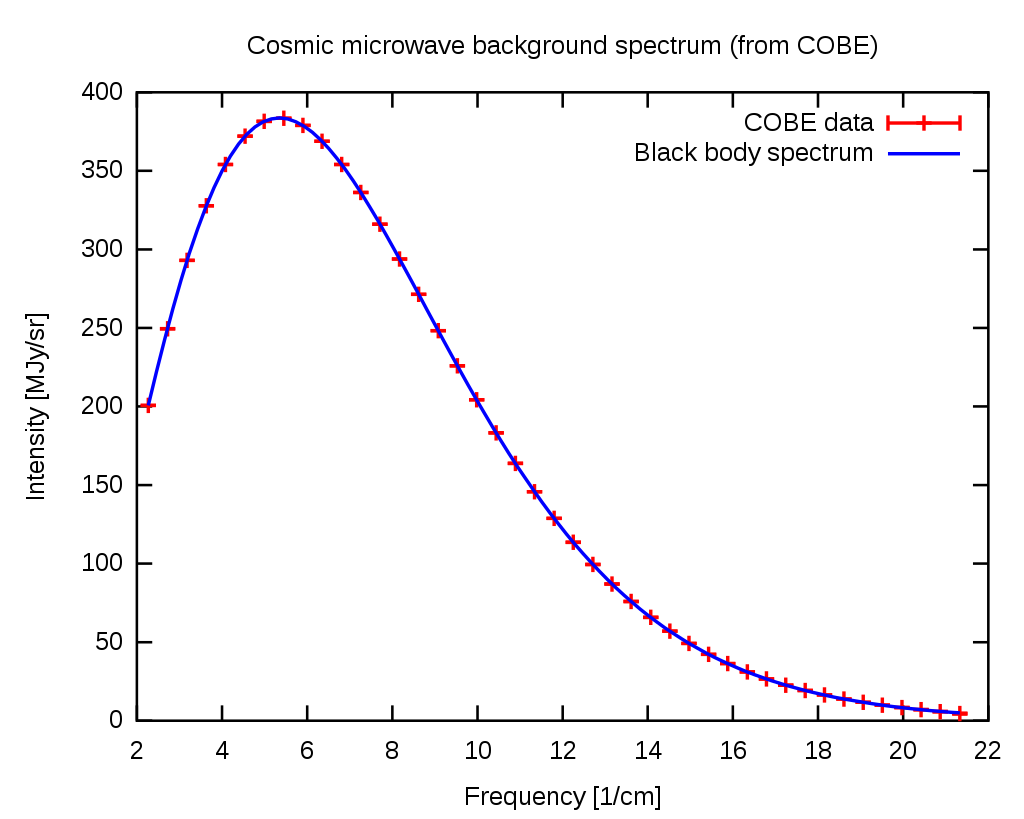
\includegraphics[width=1\textwidth]{../img/nasa_cmb_data}\\
    Images from the NASA Cobe project
    \ppagenote{CMB images from NASA (public domain)}

  \end{columns}
\end{frame}

\begin{frame}{Examples of Scientific Discoveries}{Vitamin C prevents scurvy}
  \begin{center}
    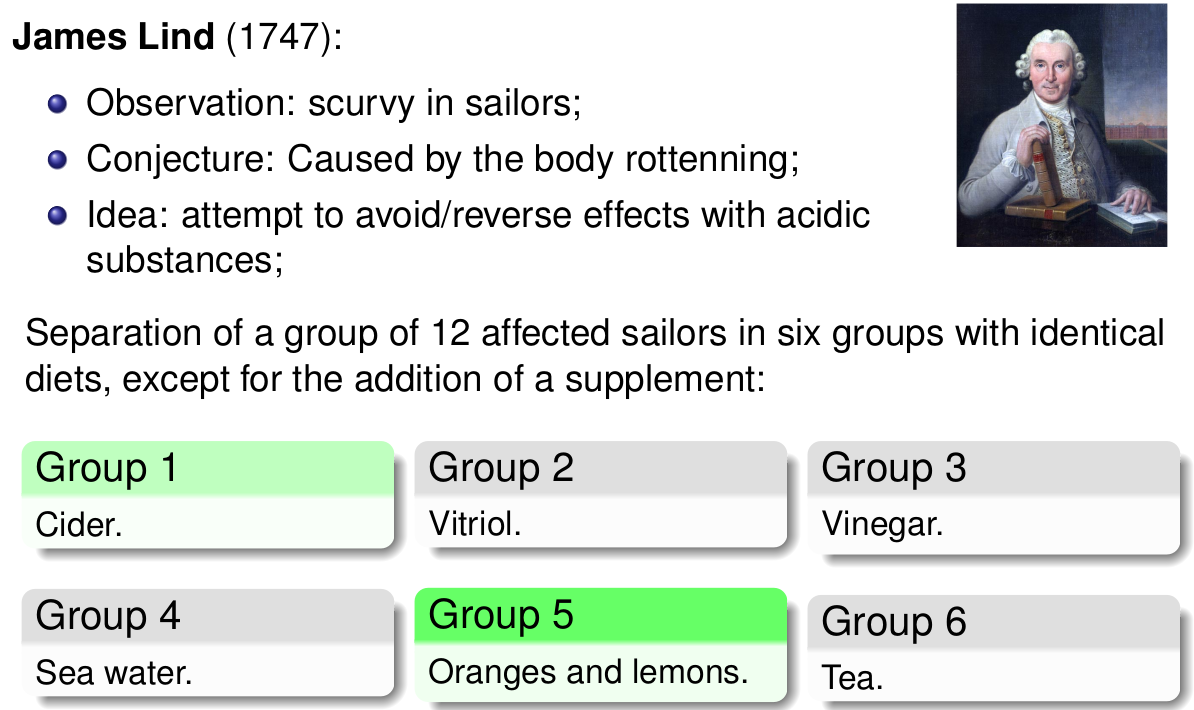
\includegraphics[width=1\textwidth]{../img/wikipedia_scurvy}
    \ppagenote{James Lind image from Wikipedia, Public Domain}
  \end{center}

\end{frame}

%% TODO: add a third example of experimentation
% Suicide contagion?
% A better example?

\subsection{The Scientific Method}
\begin{frame}{The Scientific Method}{}
  \begin{columns}
    \column{0.5\textwidth}
    \begin{itemize}
      \item The examples we saw demonstrate the familiar idea of the scientific method;
      \bigskip

      \item Hypothesis, {\bf Experiment}, Analysis;
      \bigskip

      \item But is this really all that there is to the scientific method?
    \end{itemize}
    \column{0.5\textwidth}
      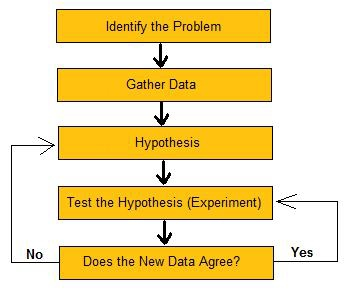
\includegraphics[width=1\textwidth]{../img/scientific_method_simple}
  \end{columns}
\end{frame}

\begin{frame}{The Scientific Method}{Science as an interactive process}
  The scientific process can be more complex than a simple recipe.
  \begin{center}
    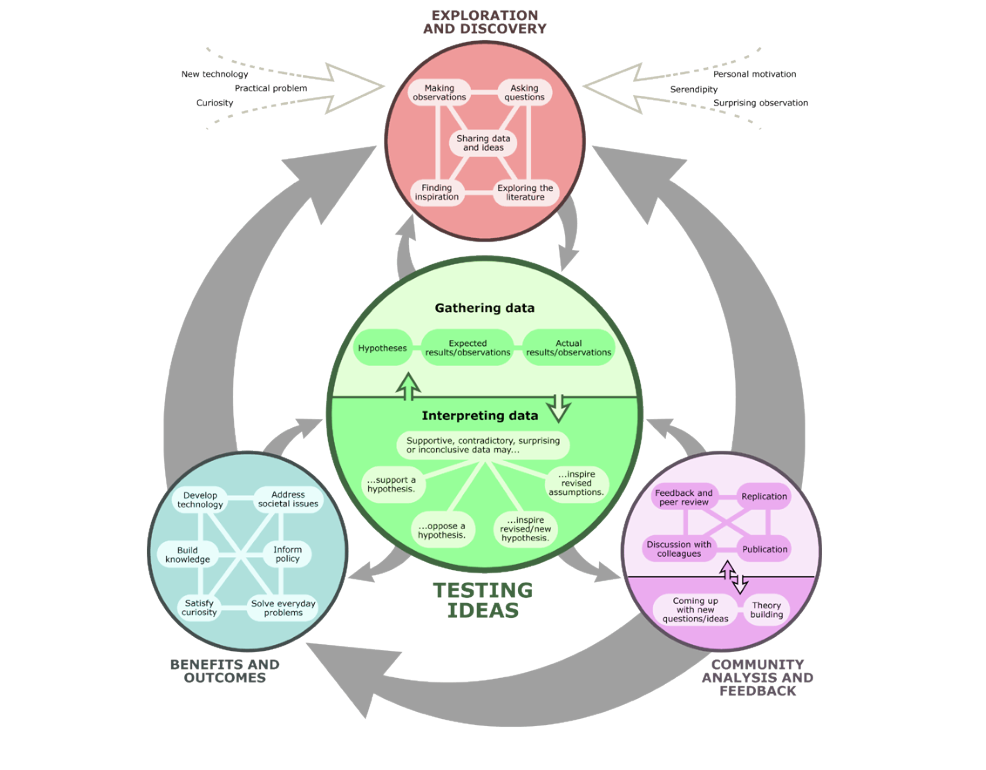
\includegraphics[width=0.7\textwidth]{../img/interactive_science}\ppagenote{Image from "understanding science, University of berkerley"}
  \end{center}
\end{frame}

\subsection{The Role of Experimentation}
\begin{frame}{The Role of Experimentation}
  \begin{itemize}
    \item Both in the simple definition of the scientific method, and on the more complete one, the experiment takes a central role;
    \bigskip

    \item An experiment is how we test hypothesis, how we learn more about the world, how we examine our ideas;
    \bigskip

    \item But what is an experiment? It is more than just collecting data!
  \end{itemize}
\end{frame}


\section{What is an Experiment?}
% Talk a little bit about Karl Popper
\begin{frame}{What is an experiment?}
  \begin{columns}[t]
    \column{0.8\textwidth}
    \begin{itemize}
      \item Philosophy of Science: How do we obtain knowledge about the world?
      \bigskip

      \item Scientific theories can only be tested by observing their implications;
      \bigskip

      \item Reject theories that cannot be confirmed by experiment;
    \end{itemize}

    \column{0.2\textwidth}
    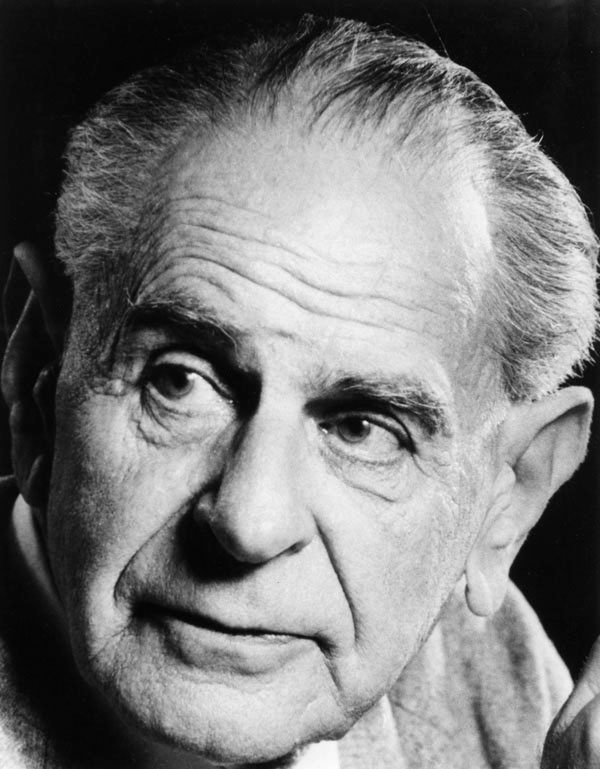
\includegraphics[width=1\textwidth]{../img/wikipedia_popper}\\
    Karl Popper (1902--1994)
    \ppagenote{Karl Popper picture from Wikipedia}
  \end{columns}
\end{frame}


\begin{frame}{What are the characteristics of a good experiment?}
  \begin{itemize}
    \item Falsifiable Hypothesis;
    \item Useful predictions;
    \item Data Collection;
    \item Reproducibility;
  \end{itemize}
\end{frame}

\begin{frame}{Falsifiability}
  \begin{center}
    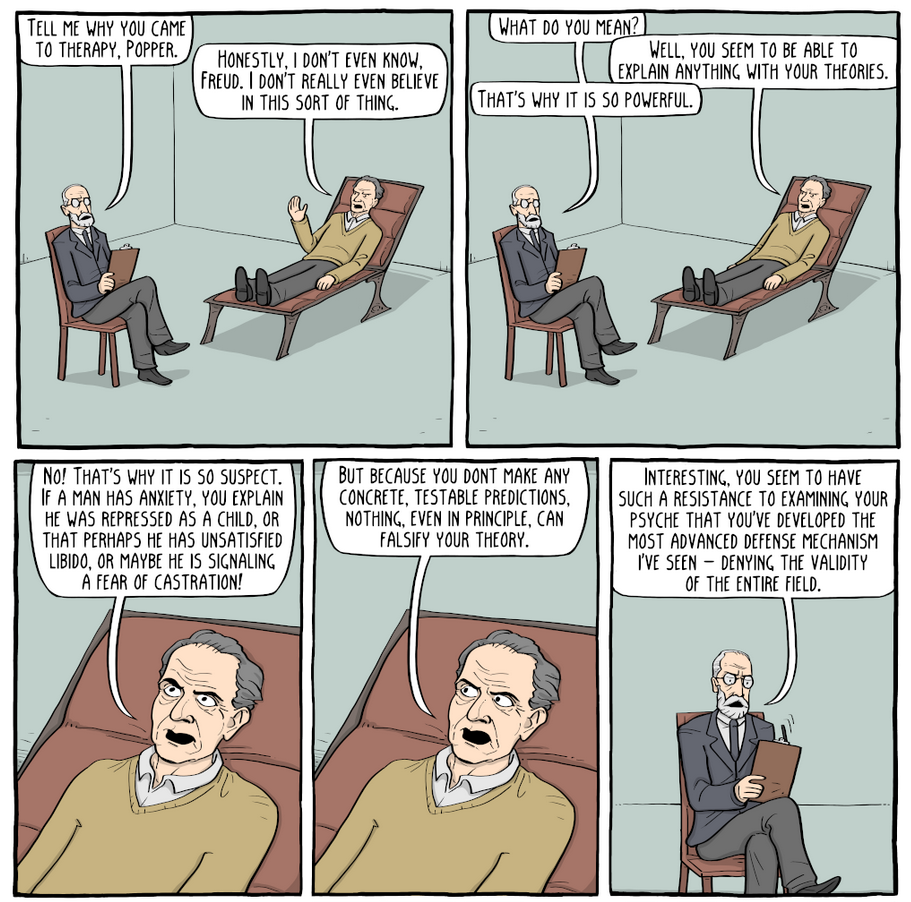
\includegraphics[width=0.7\textwidth]{../img/existentialcomics_popper}
    \ppagenote{"Froid and Popper" from \url{http://existentialcomics.com/}}
  \end{center}
\end{frame}

\begin{frame}{Falsifiability}
  \begin{columns}
    \column{0.8\textwidth}
    A scientific hypothesis is {\bf falsifiable} if there is some observation that would render it false.
    \column{0.2\textwidth}
    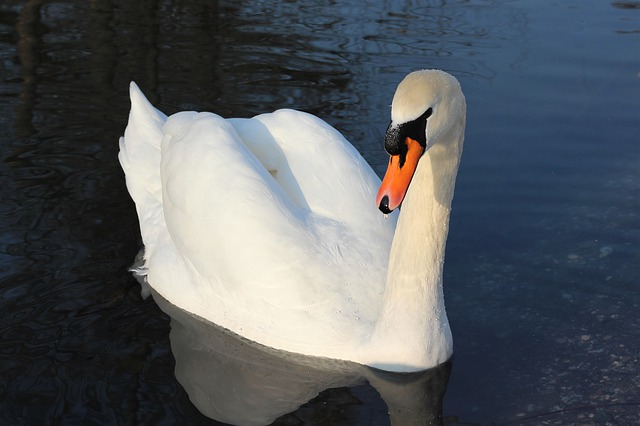
\includegraphics[width=1\textwidth]{../img/pixabay_whiteswan}
    \ppagenote{White swan image from pixabay}
  \end{columns}
  %% TODO: more specific examples
  \begin{block}{Specific Predictions}
    Falsifiable hypothesis make specific predictions about how the world behaves, not only if the hypothesis is true, but also if the hypothesis were false.
  \end{block}
  \begin{block}{Useful/Strong Predictions}
    It is not very hard to make many trivial predictions about the world. Scientific hypothesis should not only be falsifiable, but also strong and/or useful.
  \end{block}
\end{frame}

\section{Doing Experiments}
\begin{frame}{Types of Experiments}

  There are many different types of experiments, depending on what kind of data you want to obtain. Based on the data collection method, for example, we can classify an experiment in three types:
  \bigskip

  \begin{itemize}
    \item Observational Experiments;
    \item Retrospective Experiments;
    \item Controlled Experiments;
  \end{itemize}
\end{frame}
%% Three types of data collection

\begin{frame}{Types of Experiments}{Observational Experiments}
  In an \structure{Observational Experiment}, you obtain data by observing a phenomena without interacting with it directly.
  \bigskip

  {\bf Example:} you count the number of people who use the train with and without masks every day.
  \bigskip

  \begin{itemize}
    \item Requires care to observe representative situations;
    \item Allows the researcher to choose general conditions for observation;
    \item The situation of interest may be too rare to observe naturally;
  \end{itemize}
\end{frame}

\begin{frame}{Types of Experiments}{Retrospective Experiments}
  In a \structure{Retrospective Experiment}, the researcher obtains data from historical records (newspaper, reports, other scientific papers).\bigskip

  {\bf Example:} you search from the relationship between announcements of celebrity marriages, and total number of registered marriages;\bigskip

  \begin{itemize}
    \item Generally cheaper, and may be the only way to gather data over a very long period of time;
    \item Susceptible to missing records or bias in recording;
  \end{itemize}
\end{frame}

\begin{frame}{Types of Experiments}{Controlled Experiments}
  In a \structure{Controlled Experiment}, the researcher is able to define several variables in the experiment, and perform it in the conditions desired.\bigskip

  {\bf Example:} You develop a new algorithm, and test it on some selected data sets, on a collection of different computational architectures;\bigskip

  \begin{itemize}
    \item Gives a lot of control for the researcher;
    \item If not designed carefully, allows for the introduction of biases into the experiment;
    \item Can be the most expensive kind of experiment (although not always in CS);
  \end{itemize}
\end{frame}


\subsection{Experiment Design}
\begin{frame}{What is Experiment Design?}
  To perform any experiment, we have to make several technical and scientific decisions:
  \begin{itemize}
    \item Which methods we compare in the experiment?
    \item Which data sets are used?
    \item How many times do we interview each participant?
    \item In what order do we perform the experiments?
    \item Which data is reported, and how is the data summarized?
    \item What criteria determines that the hypothesis was accepted or rejected?
    \item What hyper-parameters do we use?
    \item How many times is the experiment repeated? How are these repetitions sumarized?
  \end{itemize}
  {\bf Experiment Design} is how we answer each of these questions.
\end{frame}

%% TODO: Talk a bit about design types? Educated guesses, factorial design, OVAT, etc?

\begin{frame}{Experiment Design}{Example: Controlling for Variation}
  \hfill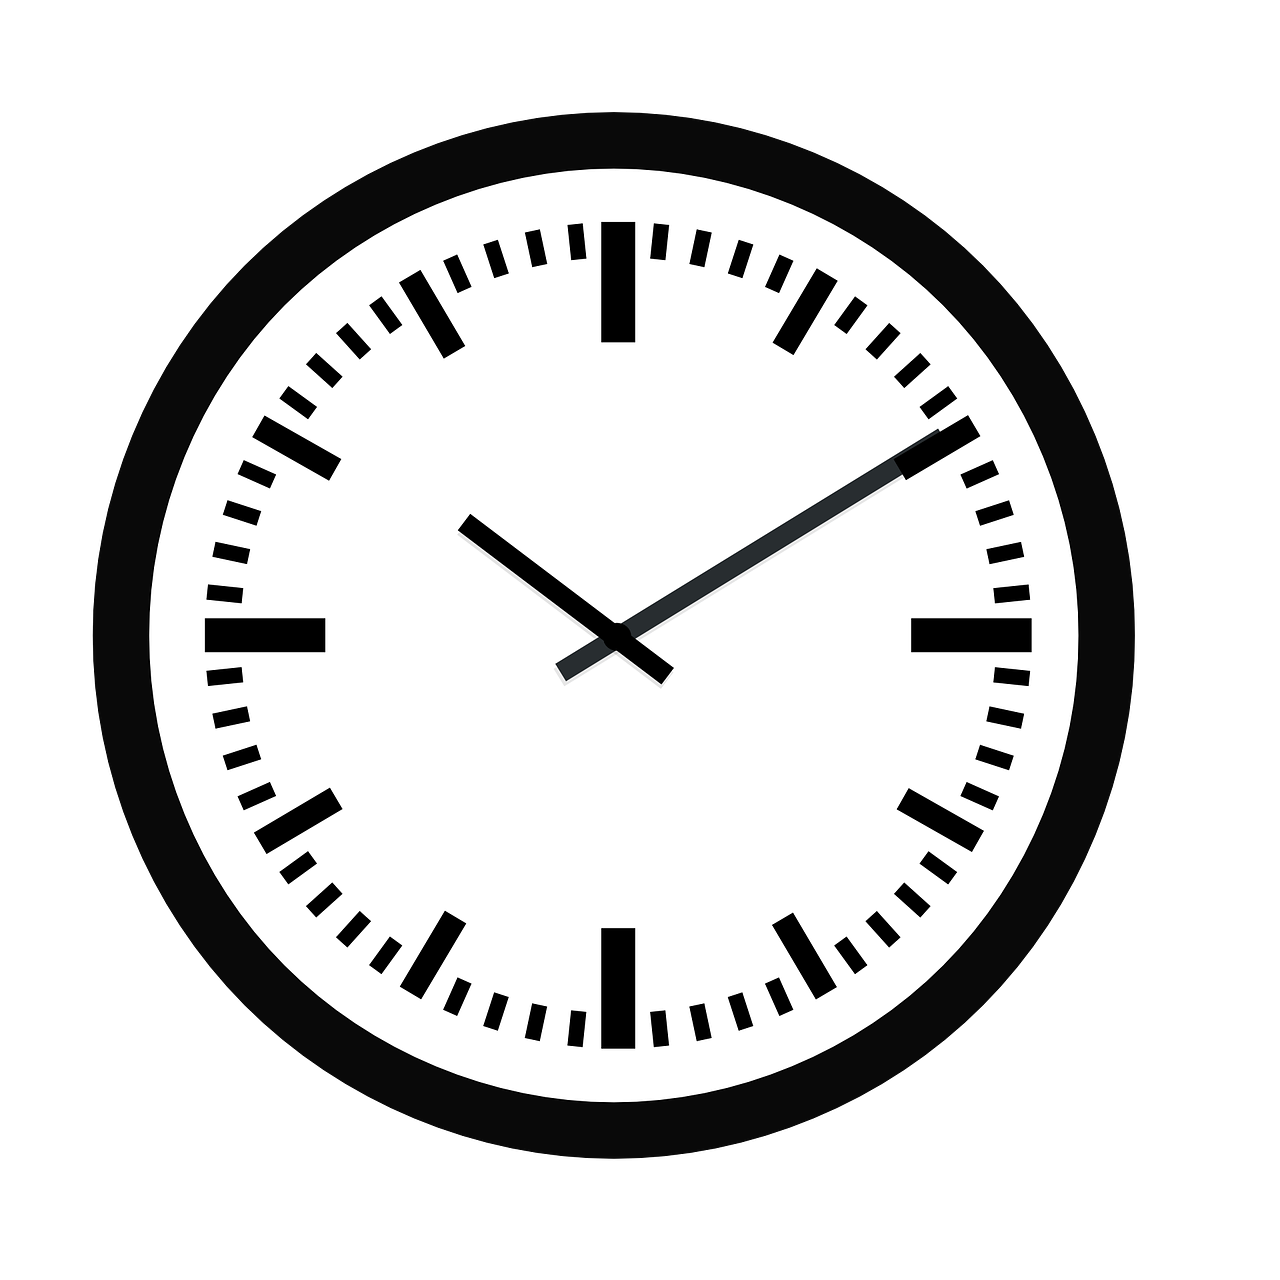
\includegraphics[width=.2\textwidth]{../img/pixabay_clock}

  Let's say you are comparing two computer programs by measuring their running time (wallclock time).
  \bigskip

  You know that the running time of a program is affected by other programs that are running in the background of the operational system. For example, if a software update happens in the background, it could make a run much slower.
  \bigskip

  To control for this variation, you make sure to run your experiment in a system with a minimum number of running processes, and you also repeat the experiment many times and take the average running time;
  \ppagenote{Clock image from \url{https://pixabay.com}}
\end{frame}

\begin{frame}{Experiment Design}{Example: Controlling for Independence}
  Imagine that you are comparing two website designs with the following experiment: You measure the time for a user to find some information on website A, then you measure the time for website B. \bigskip

  If you make this comparison always in the same order for all users, you discover that the users are a bit faster for website B, because they get used to the testing environment and are more relaxed. \bigskip

  To remove this influence, you make sure that the test order is always random, or you make sure that each user tests only one website.

  \begin{center}
    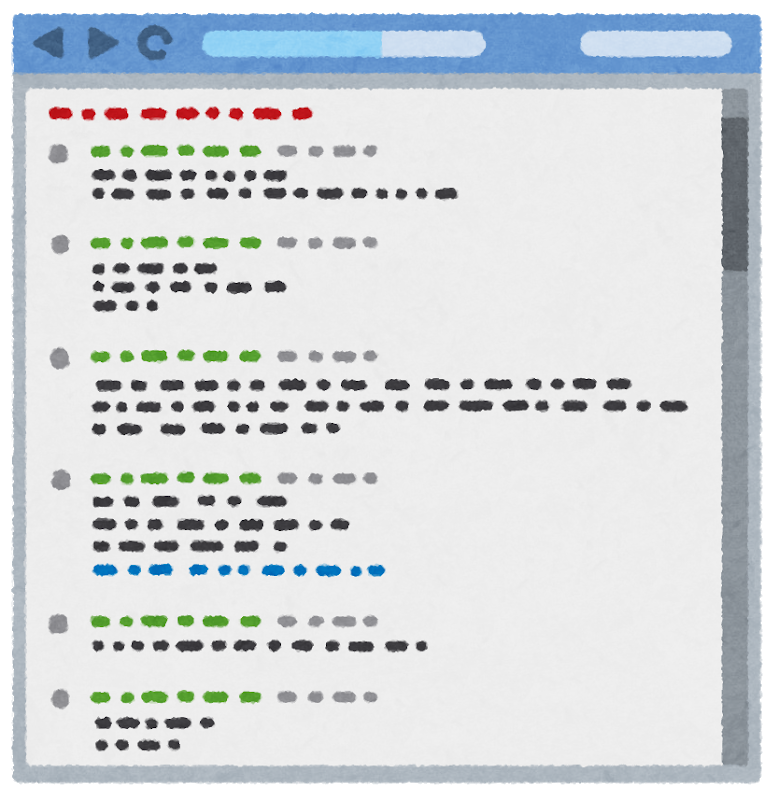
\includegraphics[width=0.2\textwidth]{../img/irasutoya_website1}\hspace{1cm}
    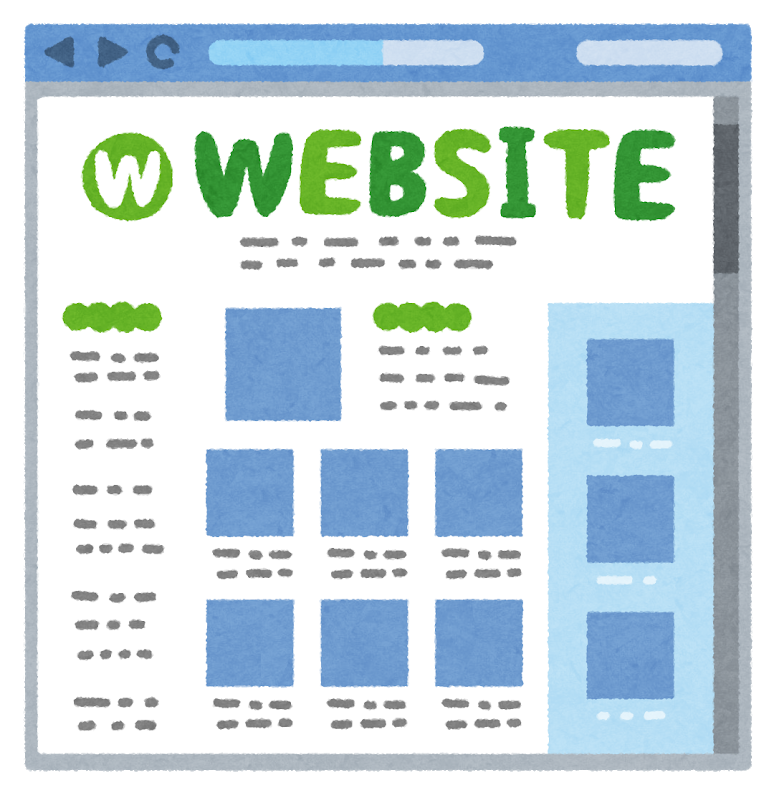
\includegraphics[width=0.2\textwidth]{../img/irasutoya_website2}
    \ppagenote{Website images from \url{https://www.irasutoya.com}}
  \end{center}
\end{frame}

\begin{frame}{Experiment Design}{Example: Controlling for Fairness}
  You propose a neural network architecture for a new vision problem, and you compare it against traditional architectures.\bigskip

  Because of the special characteristics of the problem, you fine-tune the hyper-parameters of your architecture to achieve the best performance.\bigskip

  To make sure that the comparison is fair, you use the same fine-tune techniques to the traditional architecture that you are comparing against, not using its old hyper-parameters from the literature.

  \hfill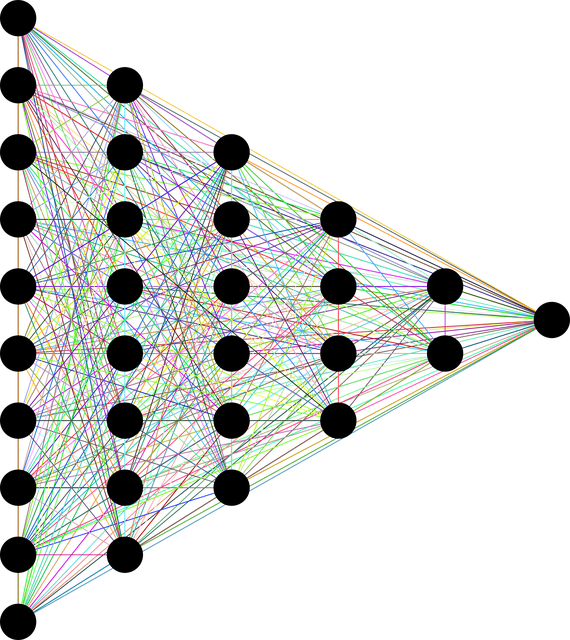
\includegraphics[width=0.2\textwidth]{../img/pixabay_neuralnetwork_gordonjohnson}
  \ppagenote{Neural Network image by Gordon Johnson from \url{https://pixabay.com}}
\end{frame}

\begin{frame}{Pre-registered Experiments}
  Pre-registration is the act of fully defining your research protocol {\bf before you begin to collect or analyse data}.
  \bigskip

  By pre-registering your research, you avoid modifying your methods to fit your hypothesis (or modifying your hypothesis to fit your data)
  \bigskip

  Public pre-registration can prevent the loss of negative results. Private pre-registration can help you keep yourself in check.\bigskip

  \begin{columns}
    \column{.7\textwidth}
    Learn more: Center for Open Science \url{https://cos.io/prereg/}
    \column{0.3\textwidth}
    
\includegraphics[width=1\textwidth]{../img/prereg-badge}
  \end{columns}
\end{frame}

\subsection{Reproducible Experiments}
\begin{frame}{Reproducible Experiments}
  Reproducibility is an important property of good research:
  \bigskip

  \begin{itemize}
    \item Others can confirm your results;
      \medskip
    \item Others can build on your results;
      \medskip
    \item Others can improve your results;
      \medskip
    \item Society can use your results;
  \end{itemize}
\end{frame}

\begin{frame}{Reproducible Experiments}{How can we make experiments more reproducible?}
  \begin{exampleblock}{Clear Experiment Design}
    Detailed steps taken to perform the experiment; Values of relevant parameters; How the results are processed and evaluated;
  \end{exampleblock}
  \begin{exampleblock}{Open Data and Open Source}
    Data acquisition protocol is clearly defined; Raw data and pre-processing scripts are available; Data is well documented;\bigskip

    For CS, open source of proposed algorithms is essential;
  \end{exampleblock}
  \begin{exampleblock}{Open Documentation}
    Code used for statistical analysis and data visualization;
  \end{exampleblock}
\end{frame}

\section{Summary}

\begin{frame}{Summary of the Lecture}
  \begin{itemize}
    \item Experimentation is a key part of Science;
    \begin{itemize}
      \item Experiments acquires data that can be used to validate or falsify scientific ideas, and to answer scientific questions;
    \end{itemize}
    \bigskip

    \item An experiment has to be performed carefully to guarantee its usefulness;
    \begin{itemize}
      \item {\bf Experimental design} defines the type of experiment, and how data is gathered;
      \item Several factors can affect the {\bf fairness and meaningfulness} of experiments;
      \item {\bf Reproducibility} is essential to guarantee the usefulness of an experiment;
    \end{itemize}
  \end{itemize}

\end{frame}

\begin{frame}{Report 1}{Design and execute a scientific experiment, and report your results}

  For this report, you must choose a simple experiment to design, perform, and analyse the results. Your report should consist of:\medskip

  \begin{itemize}
    \item {\bf Introduction}: Describe your scientific question, its relevance, and why do you need an experiment for it;
    \item {\bf Experiment Design}: Describe how you will collect data to answer your scientific question; Make sure to mention any parameters or factors that must be controlled;
    \item {\bf Data Collection:} Report on your data collection, if anything happened outside of expected from the experimental design;
    \item {\bf Analysis:} Describe your results in detail, and what answer they provide to your scientific question;
  \end{itemize}
  \begin{alertblock}{}
    \alert{Remember to follow practices of {\bf reproducible science}}
  \end{alertblock}
\end{frame}

\begin{frame}{Report 1}{How to choose an experiment for your report}
  \begin{itemize}
    \item If possible, choose something from your own research;
    \medskip

    \item Experiments from your day to day life are also good;
    \begin{itemize}
      \item Comparing cooking techniques is always fun;
      \item When collecting data, be careful of measuring errors;
    \end{itemize}
    \medskip

    \item When in doubt, comparing algorithms is an easy choice;
    \begin{itemize}
      \item Make sure to choose an appropriate metric to report!
    \end{itemize}
    \medskip

    \item Make sure you choose an experiment that you can perform!
    \bigskip

    \item Next lecture, we will talk about a bit about how to analyse and report experimental data;
  \end{itemize}
\end{frame}

\begin{frame}{Recommended Reading}
  \begin{itemize}
    \item Understanding Science \url{https://undsci.berkeley.edu/article/intro_01}
    \item Existential Comics \url{http://existentialcomics.com};
    \item Crash Course Psychology (Youtube);
  \end{itemize}
\end{frame}

%%%%%%%%%%%%%%%%%%%%%%%%%%%%%%%%%%%%%%%%%%%%%%%%%%%%
\section{Backmatter}
\begin{frame}{About these Slides}
  These slides were made by Claus Aranha, 2020. You are welcome to copy, re-use and modify this material.
  \bigskip

  These slides are a modification of "Design and Analysis of Experiments (2018)" by Felipe Campelo, used with permission.
  \bigskip

  Individual images in some slides might have been made by other
  authors. Please see the references in each slide for those cases.
\end{frame}

\begin{frame}[allowframebreaks]{Image Credits}
  \printnotes
\end{frame}

\end{CJK}
\end{document}
